% LAB 7: File I/O
%
% CSE/IT 107: Introduction to Programming
% New Mexico Tech
%
% Prepared by Russell White and Christopher Koch
% Spring 2015
\documentclass[11pt]{cselabheader}

%%%%%%%%%%%%%%%%%% SET TITLES %%%%%%%%%%%%%%%%%%%%%%%%%
\fancyhead[R]{Lab 7: File I/O}
\title{Lab 7: File I/O}

\begin{document}

\maketitle

\pagenumbering{roman}
\hrule
\begin{quotation}
``The danger that computers will become like humans is not as big as the danger
that humans will become like computers.'' (``Die Gefahr, dass der Computer so
wird wie der Mensch ist nicht so gro\ss, wie die Gefahr, dass der Mensch so wird
wie der Computer.'')
\end{quotation}
\begin{flushright}
--- Konrad Zuse
\end{flushright}

\begin{quotation}
``First, solve the problem. Then, write the code.''
\end{quotation}
\begin{flushright}
--- John Johnson
\end{flushright}

\begin{quotation}
``I don’t need to waste my time with a computer just because I am a computer
scientist.''
\end{quotation}
\begin{flushright}
--- Edsger W. Dijkstra
\end{flushright}

\hrule

\pagebreak
\section*{Introduction}
\addcontentsline{toc}{section}{Introduction}

In previous labs, we taught you how to use functions, math, lists, strings and
other features. We will combine all of these concepts in this lab and teach you
how to interact with files. You will also learn how error handling works in
Python. Some basic concepts of object oriented programming will be introduced
using turtles as an example.

\tableofcontents

\pagebreak
\pagenumbering{arabic}
\section{File I/O}
Knowing how to work with files is important, since it lets us store and retrieve
data beyond the scope of the single execution of a program. To open a file for
reading or writing we will use the \pythoninline!open()! function. The
following example opens a file named ``hello.txt'' and writes ``Hello World''
to it using the \pythoninline!print()! function.

\begin{python3code}
output_file = open("hello.txt", "w")

print("Hello World", file=output_file)
output_file.close()
\end{python3code}

The \pythoninline!print()! function can have an additional ``file'' parameter
passed to it to allow writing to a file. This causes it to send its output to
the file rather than the screen, though otherwise it performs identically.

The \pythoninline!.close()! method is used to tell Python that you are done
with a file so it can close your connection to it. If you don't call it
the file can be corrupted or other programs will be unable to access that
file.

Files can also be written to by using \pythoninline!.write(contents)!. This
method will write only the characters given to it, so a newline \lstinline{\n}
must be included for a newline.

\begin{python3code}
output_file = open("hello.txt", "w")

output_file.write("Hello World\nGoodbye!\n")
output_file.close()
\end{python3code}

The arguments to the \pythoninline!open()! function are, in order, the name of
the file to open and the mode in which to open the file. ``w'' means that the
file is to be opened in write mode. If the file does not exist, this will create
the file. If it does exist, then the contents of the file will be cleared in
preparation for the new ones.

Other options include ``a'', which is similar to ``w'' but will not clear the
contents of an existing file and will instead append the new data to the end,
and ``r'' which will read the file instead. If ``r'' is used and the file does
not exist, then an error will occur. The following code takes a filename as user
input, then prints out the entire contents of that file.

\begin{center}
  \begin{tabular}{ll}
    Mode & What it does \\
    \midrule
    a & Create file if does not exist, open file, append contents to the end \\
    w & Create or clear the file, open file, write contents to the beginning of
    file \\
    r & Open file, permit reading only \\
  \end{tabular}
\end{center}

\begin{python3code}
filename = input("What file should be read? ")

input_file = open(filename, "r")
for line in input_file:
    print(line, end="")

input_file.close()
\end{python3code}

The \pythoninline!print()! function has an additional optional ``end''
parameter. This allows you to specify what should be printed after the main
string given to it. This is important because it defaults to
\pythoninline!"\n"!, which causes a newline after every print statement. By
changing ``end'' to \pythoninline!""! we prevent a newline from being added
after every line of the file is printed. This is because each line in the
file already has a newline at the end of it, so we don't need
\pythoninline!print()! to add its own.

When reading from a file, Python can use a \pythoninline!for! loop to go
through each line in sequence. This works identically to looping through a list
of strings. Think of the file as a list with every line being a different
element of the list. The entirety of the file can also be read into a single
string using the \pythoninline!.read()! function.


This code prints the contents of a Python script.

\begin{pyconcode}
>>> input_file = open("test.py", "r")
>>> contents = input_file.read()
>>> print(contents)
filename = input("What file should be read? ")

input_file = open(filename, "r")
for line in input_file:
    print(line, end="")

input_file.close()
>>> input_file.close()
\end{pyconcode}

The \pythoninline!.readlines()! function can be used to read all of a file at
once, though it splits the file into a list. Each element of the list will be
one line of the file being read.

\subsection{Opening Files Using \protect\pythoninline!with!}
\label{sec:with}

There's an easy way to make sure every open file is closed. The
\pythoninline!with! ensures that your file is closed when the code in the
\pythoninline!with! block finished executing.

\begin{python3code}
filename = input("Enter filename: ")

with open(filename, "r") as input_file:
    for line in input_file:
        print(line, end="")
\end{python3code}

\pythoninline{input_file.close()} is not necessary because the file was closed
automatically.

\begin{warningbox}{Using \protect\pythoninline!with!}
  Always use the \pythoninline!with! statement to deal with file I/O in Python.
\end{warningbox}

\pagebreak
\section{Exceptions}

An \emph{exception} is an error message in Python. When a certain operation
encounters an error, it can \emph{raise} an exception that is then passed on to
the user. If your script is being executed as a program, exceptions cause it to
print the exception and exit.

\begin{pyconcode}
>>> 43 / 0
Traceback (most recent call last):
  File "<input>", line 1, in <module>
ZeroDivisionError: division by zero
\end{pyconcode}

However, exceptions can be handled using the \pythoninline!try!
and \pythoninline!except! statements.
The \pythoninline!except! block is only executed if an exception is caught in
the \pythoninline!try! block. Additionally, when an error is caught in the
\pythoninline!try! block we stop executing commands in the \pythoninline!try!
block and immediately jump to the \pythoninline!except! block.

The following example throws a division by zero error and prints ``division by
zero'':

\begin{python3code}
prime = 7

try:
    result = prime / 0
    result = 7 * 42
except ZeroDivisionError as err:
    print(err)
\end{python3code}

Since the error is thrown on line 5, line 6 is never executed. Also, we are
only catching \pythoninline{ZeroDivisionError} exceptions, any other exceptions
will remain uncaught.

If you are experimenting with code and want to know the name of an exception
that is thrown, take a look at the error message:

\begin{pyconcode}
>>> float('obviously not a float)
Traceback (most recent call last):
  File "<input>", line 1, in <module>
ValueError: could not convert string to float: 'obviously not a float'
\end{pyconcode}

The part highlighted in red here is the name of the error message,
\pythoninline!ValueErrror!.

Hence, if you are getting user input and want to check whether it is the
correct type, use a try-except block around the conversion:

\begin{python3code}
try:
    x = int(input('Enter an integer number: '))
except ValueError:
    print('You did not enter an integer!')
else:
    print('You entered {}'.format(x))
\end{python3code}

Notice that you can use an \pythoninline!else! block to execute code if no
exception was thrown.

Any \pythoninline!except!  block that does not list built-in exceptions will
catch all exceptions not listed in previous \pythoninline!except! blocks.
For example, the following code will throw an error if the user enters
anything but an integer:

\begin{python3code}
try:
    x = int(input("Enter a number: "))
except:
    print("Unknown error.")
    raise
else:
    print("You entered: " + str(x))
\end{python3code}

The \pythoninline!raise! keyword causes a detailed trace and prints out
additional information if an exception is encountered.  The
\pythoninline!else! block is optional and will be executed if no exceptions
are thrown in the \pythoninline!try! block.  There are many more built-in
exceptions such as \pythoninline!IOError! that can be found here:

\begin{center}
\url{https://docs.python.org/3/library/exceptions.html}
\end{center}

\subsection{File I/O Exceptions}
When working with files it is important to check for exceptions.
These are only some of the exceptions that can be raised when doing file I/O.

\begin{itemize}
  \item \pythoninline{FileNotFoundError} is raised when we try to open a file
  that. It should be handled so we can exit the program safely or recover
  rather than observe unexpected results.
  \begin{pyconcode}
>>> open("not_a_file.txt", "r")
Traceback (most recent call last):
  File "<stdin>", line 1, in <module>
FileNotFoundError: [Errno 2] No such file or directory: 'not_a_file.txt'
  \end{pyconcode}

  \item \pythoninline{IsADirectoryError} is raised when trying open an
  directory as a file.
  \begin{pyconcode}
>>> open("directory", "w")
Traceback (most recent call last):
  File "<stdin>", line 1, in <module>
IsADirectoryError: [Errno 21] Is a directory: 'directory'
  \end{pyconcode}
\end{itemize}

\pagebreak
The \pythoninline!finally! block is where clean-up actions are performed and is
always executed after leaving the \pythoninline!try! block.
The following is a good example of using \pythoninline!with! and exception
handling together to open and read a file.

\begin{python3code}
filename = input('Enter a filename >>> ')

try:
    with open(filename, 'r') as f:
        sum = 0
        for line in f:
            sum += float(line)
except FileNotFoundError:
    print('File "{}" not found'.format(filename))
except IsADirectoryError:
    print('File "{}" is a directory'.format(filename))
except ValueError:
    print('File "{}" contains a line that'.format(filename)
        + 'cannot be converted to a float')
else:
    print('Sum of all numbers in file is {}'.format(sum))
finally:
    print('Goodbye.')
\end{python3code}

\pagebreak
\section{Using Objects: Creating Turtles}
We have been implicit using two important definitions. These are part of object
oriented programming, which will be covered in more detail in later labs.
\begin{description}
  \item[Object] is a Python data type that can contain arbitrary amounts and
  kinds of data. They can be instantiated or created in several ways. Some
  examples:

  \begin{description}
    \item[\pythoninline{int}, \pythoninline{str}, \pythoninline{list}] Built-in
    types are objects and are created by writing literals such as
    \pythoninline{1}, \pythoninline{"Hello"}, \pythoninline{[1,2,3]} or by
    conversion \pythoninline{list("123")}.
    \item[\pythoninline{file}] Files are also objects. They are created using
    the \pythoninline{open()} function.
    \item[\pythoninline{Exception}] Exceptions are objects created when they
    are \pythoninline{raise}d.
    \item[\pythoninline{Turtle}] These are created by calling
    \pythoninline{turtle.Turtle()}.
  \end{description}
  \item[Method] is a function that is specific a certain object. Some examples
  include \pythoninline{str.find()}, \pythoninline{list.reverse()},
  \pythoninline{file.write()}, \pythoninline{Turtle.forward()},
  \pythoninline{Exception.err()}.
\end{description}

Knowing this, we can create multiple turtles and draw more complex designs.
This is done by instantiating new turtles with the
\pythoninline!turtle.Turtle()! function. This function returns a turtle
object, which we can call every other normal turtle method on.

\begin{python3code}
import turtle

first = turtle.Turtle()
second = turtle.Turtle()

first.forward(50)
second.forward(50)
first.left(90)
second.right(90)
first.forward(50)
second.forward(50)
first.right(90)
second.left(90)
first.forward(50)
second.forward(50)
\end{python3code}

\begin{figure}[h]
  \centering
  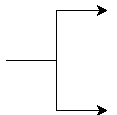
\includegraphics[width=1.0in]{img/turtle_prong}
\end{figure}

If we add a group of turtles to a list, we can easily apply the same commands to all of them, as in this example:

\begin{python3code}
import turtle

turtles = []
first = turtle.Turtle()
first.speed(0)
turtles.append(first)

second = turtle.Turtle()
second.speed(0)
second.right(90)
turtles.append(second)

third = turtle.Turtle()
third.speed(0)
third.right(180)
turtles.append(third)

fourth = turtle.Turtle()
fourth.speed(0)
fourth.right(270)
turtles.append(fourth)

for i in range(200):
    for turt in turtles:
        turt.forward(i/5)
        turt.left(10)
\end{python3code}

\begin{figure}[h]
  \centering
  
\includegraphics[width=0.6\textwidth]{img/fancy_spiral}
\end{figure}


% \begin{figure}[h]
%   \centering
%   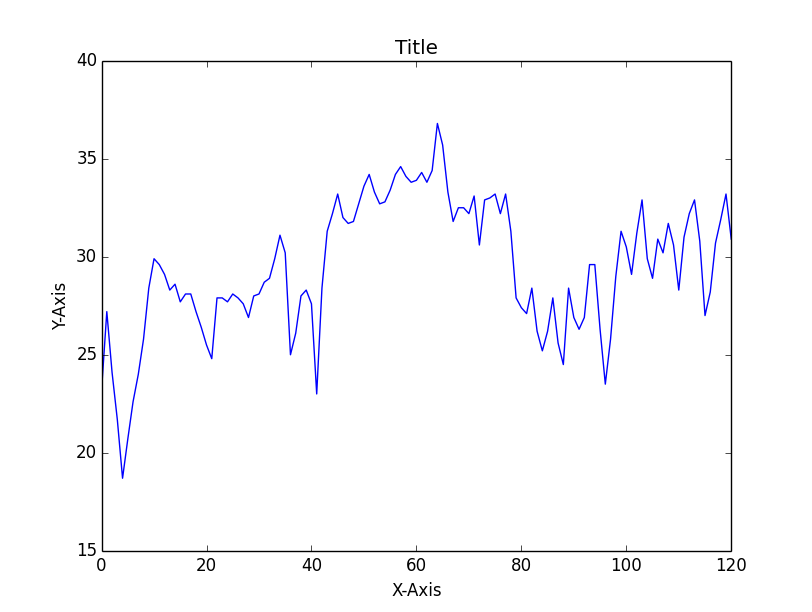
\includegraphics[width=0.85\textwidth]{img/line1.png}
%   \caption{Line plot example: temperature data from Tucson, AZ.}
%   \label{fig:line1}
% \end{figure}
%
% The following code will show a line plot of the dataset. You can see the graph
% it produces in Figure~\ref{fig:line1}.
%
% \begin{python3code}
% import matplotlib.pyplot as plt
%
% with open("2cities.csv", "r") as f:
%     lines = f.readlines()
%
% temps = []
% for line in lines:
%     cols = line.split()
%     try:
%         if len(cols) > 1:
%             temps.append(float(cols[1]))
%     except ValueError:
%         pass # could not convert to float, must be first row with headers
%
% plt.plot(list(range(len(temps))), temps)
% plt.xlabel("Data point")
% plt.ylabel("Temperature in degrees Celsius")
% plt.title("Temperature in Tucson, AZ over 120 days")
% plt.show()
% \end{python3code}
%
% Next, we are trying to create a histogram of the data.
%
% \begin{itemize}
%   \item A histogram is a bar graph where a bar represents
%     a temperature \emph{range}. We call one of these ranges a bin or a bucket.
%   \item
%     For example, the temperatures in Tucson in the data set
%     range from 18$^\circ$ Celsius to 37$^\circ$ Celsius. We would create a
%     histogram spanning temperatures from $15^\circ$ to $40^\circ$ Celsius with
%     bins of size $5^\circ$ Celsius. That means a bin for $15$ to $20$ degrees
%     Celsius, a bin for $20$ to $25$ degrees Celsius, etc.
% \end{itemize}
%
% \begin{python3code}
% import matplotlib.pyplot as plt
%
% with open("2cities.csv", "r") as f:
%     lines = f.readlines()
%
% temps = []
% for line in lines:
%     # columns in 2cities.csv are [data point number, tucson temp, eugene temp]
%     cols = line.split()
%     try:
%         if len(cols) > 1:
%             temps.append(float(cols[1]))
%     except ValueError:
%         pass # could not convert to float, must be first row with headers
%
% numbuckets = 5
% binnumbers = range(0, numbuckets)
% counts = []
% for bucketno in binnumbers:
%     bucket = []
%     for temp in temps:
%         if 15 + bucketno * 5 < temp < 15 + (bucketno + 1) * 5:
%             bucket.append(temp)
%     # Count how many temperatures are in this bucket.
%     # This count will be the height of the bar in the graph.
%     counts.append(len(bucket))
%
% xlabels = []
% for bucket in binnumbers:
%     xlabels.append("{} to {}C".format(15 + bucket * 5, 15 + (bucket + 1) * 5))
%
% plt.bar(binnumbers, counts, align="center")
% plt.xticks(binnumbers, xlabels)
% plt.xlabel("Temperature in Celsius")
% plt.ylabel("Number of times occured")
% plt.title("Histogram of Temperatures in Tucson, AZ")
% plt.show()
% \end{python3code}
%
% This code will produce this output of the input data sorted into 10 bins of size
% 5 (not showing empty bins) as seen Figure~\ref{fig:bar1}.
%
% \begin{figure}[h]
%   \centering
%   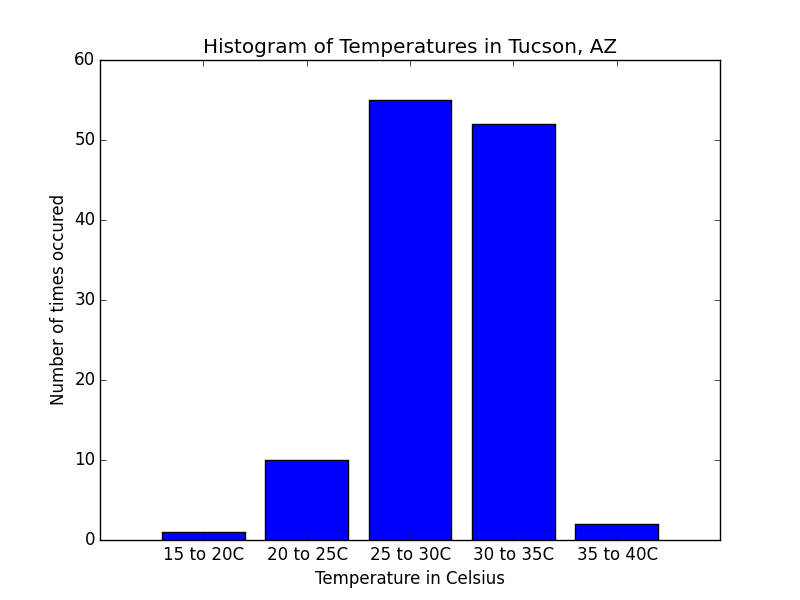
\includegraphics[width=0.85\textwidth]{img/histo_tucson.png}
%   \caption{Input data sorted into 5 bins of size 5$^\circ$ Celsius.}
%   \label{fig:bar1}
% \end{figure}
%
% \subsection{More Documentation}
%
% \begin{itemize}
%   \item \pythoninline!.plot()! function documentation:
%     \begin{center}
%       \url{http://matplotlib.org/api/pyplot\_api.html#matplotlib.pyplot.plot}
%     \end{center}
%   \item \pythoninline!.bar()! function documentation:
%     \begin{center}
%       \url{http://matplotlib.org/api/pyplot\_api.html#matplotlib.pyplot.bar}
%     \end{center}
%   \item Documentation overview for \pythoninline{matplotlib.pyplot}:
%     \begin{center}
%       \url{http://matplotlib.org/api/pyplot\_summary.html}
%     \end{center}
% \end{itemize}

\pagebreak
\section{Exercises}
\label{sec:ex}

\begin{warningbox}{Using \protect\pythoninline!with!}
  Always use the \pythoninline!with! statement to deal with file I/O in Python.
  See Section~\ref{sec:with}.
\end{warningbox}

\begin{ex}[save.py] Write a program that takes in a filename, then takes in
  a series of lines of input until a blank line is entered, writing each line to
  the file with the given name. After the blank line is entered, properly close
  the file before ending the program.
\end{ex}

\begin{ex}[word\_count.py] Write a program that
  takes in a filename and string as input. Then print how many times that string
  appears inside the chosen file. If the file does not exist, continue asking
  for a filename until one is given that exists. Use your source code file as
  test input. Make sure to test lines contain the same word multiple times.
\end{ex}

\begin{ex}[diff.py]
  Write a ``diff'' program that prints out the differences, line by line, of
  two files.  Your program should ask the user for the names of two files,
  then print the differences between them.  Follow the format output as shown
  below. Make sure to use proper error handling techniques for file I/O.

  Example:

  \begin{listing}[H]
    \vspace{-0.5em}
    \begin{verbatimcode}
John goes to work.
Keith and Kyle went to the Ensiferum concert.
Alice ate an apple pie.
Joe cut down a tree.
The dog jumped over the wall.
    \end{verbatimcode}
    \vspace{-0.5em}
    \caption{file1.txt}
    \vspace{-0.5em}
  \end{listing}

  \begin{listing}[H]
    \vspace{-0.5em}
    \begin{verbatimcode}
John goes to work.
Coral went to a Kesha concert.
Alice ate an apple pie.
Joe planted a tree.
The dog jumped over the wall.
    \end{verbatimcode}
    \vspace{-0.5em}
    \caption{file2.txt}
    \vspace{-0.5em}
  \end{listing}

  \begin{verbatimcode}
Enter file name 1 >>> file1.txt
Enter file name 2 >>> file2.txt

2c2
< Keith and Kyle went to the Ensiferum concert.
---
> Coral went to a Kesha concert.
4c4
< Joe cut down a tree.
---
> Joe planted a tree.
  \end{verbatimcode}
\end{ex}

\begin{ex}[readscores.py]
  Download the file \texttt{actsat.txt} provided on Canvas. It contains the
  following columns of tab-separated data:

  \begin{enumerate}[\text{Column} 1~]
    \item 2-letter state/territory code (includes DC)
    \item \% of graduates in that state taking the ACT
    \item Average composite ACT score
    \item \% of graduates in that state taking the SAT
    \item Average SAT Math score
    \item Average SAT Reading score
    \item Average SAT Writing score
  \end{enumerate}

  You must open this file and generate a list of dictionaries containing each
  row of data. Please use these keys for the dictionaries:
  \begin{multicols}{3}
  \begin{itemize}
  \item \pythoninline{"state"}
  \item \pythoninline{"act_percent_taking"}
  \item \pythoninline{"act_average_score"}
  \item \pythoninline{"sat_percent_taking"}
  \item \pythoninline{"sat_average_math"}
  \item \pythoninline{"sat_average_reading"}
  \item \pythoninline{"sat_average_writing"}
  \end{itemize}
  \end{multicols}

  For example, if you get this two line data file your code should
  form the following list of dictionaries.

  \begin{verbatimcode}
AK      27      21.2    48      517     519     491
AL      81      20.3    9       556     563     554
  \end{verbatimcode}

  \begin{python3code}
[{"state": "AK",
  "act_percent_taking":  27
  "act_average_score":   21.2
  "sat_percent_taking":  48
  "sat_average_math":    517
  "sat_average_reading": 519
  "sat_average_writing": 491
 },
 {"state": "AK",
  "act_percent_taking":  81
  "act_average_score":   20.3
  "sat_percent_taking":  9
  "sat_average_math":    556
  "sat_average_reading": 563
  "sat_average_writing": 554
}]
  \end{python3code}
\end{ex}

\section{Submitting}

You should submit your code as a tarball. It should contain all files
used in the exercises for this lab. The submitted file should be named
\begin{center}
  \texttt{cse107\_firstname\_lastname\_lab7.tar.gz}
\end{center}

\begin{center}
  \textbf{Upload your tarball to Canvas.}
\end{center}

\listofexercises

\end{document}













